\section{AoA}

    \subsection{Chegada do sinal}
    \begin{frame}{\textit{Angle of Arrival}}
        \begin{figure}
            \centering
            \caption*{$ \theta_\text{AoA} = \SI{60}{\degree} $, $\textcolor{cmyk_M}{\alpha_{k}}=\SI{20}{\degree}$, $ \textcolor{Purple}{\beta_{\pm k}} = \SI{40}{\degree} $}
            % % \resizebox{!}{0.7\textheight}{%
\begin{circuitikz}[american, voltage shift=0.5, line width=0.5, every node/.style={font = {\footnotesize\bfseries}}]

    \def\wavelength{3.5}
    \pgfmathsetmacro\d{0.5*\wavelength}

    \def\antennaAngle{20}
    \pgfmathsetmacro\signalAngle{\antennaAngle+40}

    \def\closeRange{9}
    \def\farRange{\closeRange+13}

	\def\NAntennas{3}
	\pgfmathsetmacro\AngleAntennas{360/\NAntennas}
	\def\ShiftAngleAntennas{-90}

	\pgfmathsetmacro\RhoAntennas{\d/(2*sin(180/\NAntennas))}

    \def\centerarc(#1)(#2:#3:#4)% Syntax: [draw options] (center) (initial angle:final angle:radius)
    { ($(#1)+({#4*cos(#2)},{#4*sin(#2)})$) arc (#2:#3:#4) }

    \def\coordref[#1](#2){%

        \coordinate(sysref) at (#2);

        \draw[#1, -latex] (sysref) ++(-0.4,-0.3) -- ++(0.9,0) node[midway, below]{$x$};
        \draw[#1, -latex] (sysref) ++(-0.3,-0.4) -- ++(0,0.9) node[midway, left]{$y$};
        \draw[#1, -latex] \centerarc(sysref)(-90:180:0.25);
        \draw[#1] (sysref) node{$+$}
    }

    \coordinate (bottomleft) at (-3.5,-1);
    \coordinate (topright) at (3.5,5);


    % \draw[Red,dashed] (bottomleft) rectangle (topright);
    \clip (bottomleft) rectangle (topright);

    \coordinate (O) at (0,0);
    \coordinate (sourceAntenna) at (\signalAngle:\closeRange*\wavelength);
    % \draw [help lines, dashed] (bottomleft) grid (topright); % desenha grid
    % \draw [red] (O) node[draw,cross out] {}; % marca pont(0,0)

    % Circulo de antenas
	% \draw[densely dotted, opacity=0.25] (O) ++(90:\RhoAntennas) circle (\RhoAntennas);

    % Linhas do sinal de fundo
    \foreach \x [evaluate={\y=int((\x+\closeRange));\z=int((\x+\closeRange));}] in {-3,...,3} {
        \draw [black!75, very thin]
        (sourceAntenna) ++ (\signalAngle:-\z*\wavelength)
            % node[anchor=west, font = {\footnotesize\bfseries}]{$\y\lambda$}
        ($(sourceAntenna) + (\signalAngle:-\z*\wavelength) + ({10*cos(\signalAngle+90)},{10*sin(\signalAngle+90)})$)
            --
        ($(sourceAntenna) + (\signalAngle:-\z*\wavelength) - ({10*cos(\signalAngle+90)},{10*sin(\signalAngle+90)})$)
        % \draw [gray, thin] (sourceAntenna) circle (\z)
        ;
    }

    % Antenas
    \draw[thick, cmyk_R] (O) node[dinantenna] (A00) {} ;
    % \draw[thick, cmyk_G, opacity=0.75] (O) ++(60:\d) node[dinantenna] (A0d) {} node [below] {$A_{k+2}$};
    \draw[thick, cmyk_B] (O) ++(\antennaAngle:\d) node[dinantenna] (Ad0) {} ;

    \draw[very thin, Black!50, -latex] % Desenha eixo X
        (-3,0) -- (3,0) node[below left] {$x$}
    ;

    % Ângulo alpha entre antenas
    \draw[thin, cmyk_M]
        \centerarc(O)(0:\antennaAngle:0.3)
        node [above, inner sep=3pt] {$\alpha$}
    ;


    % Desenha senoide de fundo
    \draw[Goldenrod, domain=-8:8, samples=100]
        (A00) ++(\signalAngle+90:0.5*\wavelength) coordinate(signalAux)
        plot[shift={(signalAux)}, rotate=\signalAngle]({\x},{cos(\x * pi * 2 / \wavelength r)})
    ;

    % Direção do sinal
    \draw[very thick, dashed, -latex, Goldenrod]
        % (A00) ++(1.5*\d,0) ++ (\signalAngle:-0.5*\d) -- coordinate(angleArrow) ++(\signalAngle:\d)
        (A00) ++(-2,0) ++ (\signalAngle:-0.25*\d) -- coordinate(angleArrow) ++ (\signalAngle:0.5*\d) --++(\signalAngle:0.25*\d)
    ;
    % Angulo Theta do sinal
    \draw[thin]
        (angleArrow) ++ (0.4, 0) node [below,inner sep=2pt] {$\theta_\text{\ac{AoA}}$}
        \centerarc(angleArrow)(0:\signalAngle:0.4)
    ;

    % Triangulo retângulo + quadradinho
    \draw[Black]

        (A00) --++($({\signalAngle-90}:{\d*sin(\signalAngle-\antennaAngle)})$) coordinate (pontoTriangulo) -- (Ad0) -- (A00)

        (pontoTriangulo)
          ++(\signalAngle:0.125)
        --++(\signalAngle+90:0.125)
        --++(\signalAngle+180:0.125)
    ;

    % Arco do angulo beta
    \draw[thin, Purple]
        (Ad0) ++ (180+\antennaAngle:0.4) node[above, inner sep=3pt] {$\beta$}
        \centerarc(Ad0)(180+\antennaAngle:180+\signalAngle:0.4)
    ;

    % Distânci d entre antenas
    \draw[latex-latex]
        ($(A00)+(0,1)$) -- ($(Ad0)+(0,1)$) node [midway, fill=white, circle, inner sep=1pt] {$d$}
    ;

    \newcommand\CircleRadius{3cm}
    %   \draw (0,0) circle (\CircleRadius);
    % special method of noting the position of a point
    \coordinate (P) at (50:\CircleRadius);

\end{circuitikz}
% }


            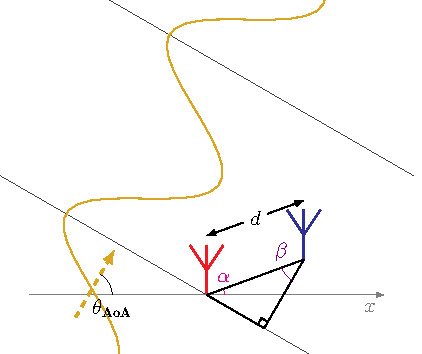
\includegraphics{../pictures/AoA_1}
            \caption*{\usebeamercolor[fg]{palette sidebar tertiary} \tiny Fonte: Autor.}
        \end{figure}
    \end{frame}

    \begin{frame}{\textit{Angle of Arrival}}
        \begin{figure}
            \centering
            \caption*{$ \theta_\text{AoA} = \SI{-20}{\degree} $, $\textcolor{cmyk_M}{\alpha_{k}}=\SI{20}{\degree}$, $ \textcolor{Purple}{\beta_{\pm k}} = \SI{40}{\degree} $}
            %     % \resizebox{!}{0.7\textheight}{%
    \begin{circuitikz}[american, voltage shift=0.5, line width=0.5,every node/.style={font = {\footnotesize\bfseries}}]

        \def\wavelength{3.5}
        \def\d{0.5*\wavelength}

        \def\antennaAngle{210}

        \def\closeRange{9}
        \def\farRange{\closeRange+13}

        \def\centerarc[#1](#2)(#3:#4:#5)% Syntax: [draw options] (center) (initial angle:final angle:radius)
        { \draw[#1] ($(#2)+({#5*cos(#3)},{#5*sin(#3)})$) arc (#3:#4:#5) node[midway,anchor=west] {$\beta$}; }


        \coordinate (O) at (0,0);
        \coordinate (antenna) at (\antennaAngle:\closeRange*\wavelength);
        % \draw [help lines, dashed] (-5,-3) grid (5,3); % desenha grid
        % \draw [red] (O) node[draw,cross out] {}; % marca pont(0,0) 
        
        % \draw (-6.8,-4) rectangle (6.8,4);
        \clip (-3.5,-3.5) rectangle (3.5,3.5);

        % \draw[thick]
        %     (antenna) node[dinantenna]{}
        % ;
        
        \foreach \x [evaluate={\y=int((\x+\closeRange));\z=int((\x+\closeRange));}] in {-3,...,3} {
            \draw [black, thin] 
            (antenna) ++ (\antennaAngle:-\z*\wavelength)
                % node[anchor=west, font = {\footnotesize\bfseries}]{$\y\lambda$}
            ($(antenna) + (\antennaAngle:-\z*\wavelength) + ({10*cos(\antennaAngle+90)},{10*sin(\antennaAngle+90)})$)
                -- 
            ($(antenna) + (\antennaAngle:-\z*\wavelength) - ({10*cos(\antennaAngle+90)},{10*sin(\antennaAngle+90)})$);
            % \draw [gray, thin] (antenna) circle (\z);
        }
        
        \draw[thick]
            (0,0)  node[Green, dinantenna] (A00) {}
            % (0,\d) node[Blue,  dinantenna] (A0d) {}
            (\d,0) node[Red,   dinantenna] (Ad0) {}
        ;

        \draw[very thick, dashed, -latex]
            (A00) ++(-\d,0) coordinate(aux) ++(\antennaAngle:0.5*\d) -- ++(\antennaAngle:-\d)
        ;

        
        \draw[Goldenrod, domain=-8:8, samples=100] plot[shift={(aux)}, rotate=\antennaAngle]({\x},{sin(\x * pi * 2 / \wavelength r)});
        
        \draw[thin, opacity=0.5]
            (A00) ++ ($({\antennaAngle-90}:{\d*sin(\antennaAngle)})$) -- (Ad0) -- (A00)

            ($({\antennaAngle-90}:{\d*sin(\antennaAngle)})$) 
              ++(\antennaAngle+180:0.125)
            --++(\antennaAngle-90:0.125)
            --++(\antennaAngle:0.125)

            
        ;

        \centerarc[thin, opacity=0.5](A00)(\antennaAngle+90:360:0.4)

        \draw[latex-latex]
            ($(A00)+(0,1)$) -- ($(Ad0)+(0,1)$) node [midway, fill=white] {$d$}
        ;
        


        % \foreach \x in {0,60,...,300} {
        %     \draw[thick] (\x:1 cm) -- (\x + 60:1 cm);
            
        %     \draw (\x + 30:1.732 cm) node[Gray, circ]{};
        %     \draw[Gray, dashed] (\x:1 cm) -- ++(\x: 0.9cm);
        %     \draw[Gray, dotted]
        %     %     % (\x:1 cm) arc (\x+240:\x+180:1cm)
        %         (\x:1 cm) arc [start angle=\x+120, delta angle=110, radius=1cm]
        %         (\x:1 cm) arc [start angle=\x+120, delta angle=-50, radius=1cm]
        %     ;
        % }
    
        % \draw (0,0) node [circ] {} node [below left,font={\scriptsize\bfseries}] {BS};
        % \draw[thick, densely dotted] (0,0) circle (1cm);
        
        % \draw[-latex] (0,0) -- (0:1cm) node[midway, below] {$R_c$};
        % \draw[-latex] (0,0) -- (90:0.866cm) node[midway, left] {$R$};
            
    \end{circuitikz}
  % }


            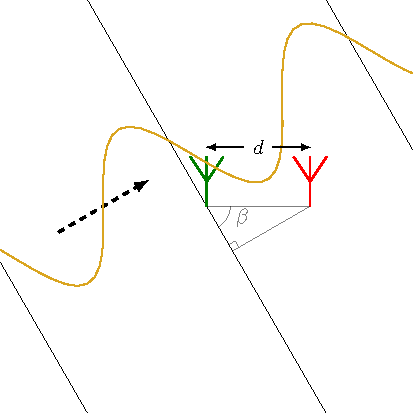
\includegraphics{../pictures/AoA_2}
            \caption*{\usebeamercolor[fg]{palette sidebar tertiary} \tiny Fonte: Autor.}
        \end{figure}
    \end{frame}

    \begin{frame}{\textit{Angle of Arrival}}
        \begin{figure}
            \centering
            \caption*{$ \theta_\text{AoA}=\SI{110}{\degree} $, $\textcolor{cmyk_M}{\alpha_{k}}=\SI{20}{\degree}$, $ \textcolor{Purple}{\beta_{\pm k}} = \SI{90}{\degree} $}
            %     % \resizebox{!}{0.7\textheight}{%
    \begin{circuitikz}[american, voltage shift=0.5, line width=0.5,every node/.style={font = {\footnotesize\bfseries}}]

        \def\wavelength{3.5}
        \def\d{0.5*\wavelength}


        \def\antennaAngle{180}
        \def\closeRange{9}
        \def\farRange{\closeRange+13}

        \def\centerarc[#1](#2)(#3:#4:#5)% Syntax: [draw options] (center) (initial angle:final angle:radius)
        { \draw[#1] ($(#2)+({#5*cos(#3)},{#5*sin(#3)})$) arc (#3:#4:#5) node[midway,anchor=west] {$\beta$}; }


        \coordinate (O) at (0,0);
        \coordinate (antenna) at (\antennaAngle:\closeRange*\wavelength);
        % \draw [help lines, dashed] (-5,-3) grid (5,3); % desenha grid
        % \draw [red] (O) node[draw,cross out] {}; % marca pont(0,0) 
        
        % \draw (-6.8,-4) rectangle (6.8,4);
        \clip (-3.5,-3.5) rectangle (3.5,3.5);

        % \draw[thick]
        %     (antenna) node[dinantenna]{}
        % ;
        
        \foreach \x [evaluate={\y=int((\x+\closeRange));\z=int((\x+\closeRange));}] in {-3,...,3} {
            \draw [black, thin] 
            (antenna) ++ (\antennaAngle:-\z*\wavelength)
                % node[anchor=west, font = {\footnotesize\bfseries}]{$\y\lambda$}
            ($(antenna) + (\antennaAngle:-\z*\wavelength) + ({10*cos(\antennaAngle+90)},{10*sin(\antennaAngle+90)})$)
                -- 
            ($(antenna) + (\antennaAngle:-\z*\wavelength) - ({10*cos(\antennaAngle+90)},{10*sin(\antennaAngle+90)})$);
            % \draw [gray, thin] (antenna) circle (\z);
        }
        
        \draw[thick]
            (0,0)  node[Green, dinantenna] (A00) {}
            % (0,\d) node[Blue,  dinantenna] (A0d) {}
            (\d,0) node[Red,   dinantenna] (Ad0) {}
        ;

        \draw[very thick, dashed, -latex]
            (A00) ++(-\d,0) coordinate(aux) ++(\antennaAngle:0.5*\d) -- ++(\antennaAngle:-\d)
        ;

        
        \draw[Goldenrod, domain=-8:8, samples=100] plot[shift={(aux)}, rotate=\antennaAngle]({\x},{cos(\x * pi * 2 / \wavelength r)});
        % \draw[thin, densely dotted]
        %     (A00) ++ ($({\antennaAngle-90}:{\d*sin(\antennaAngle)})$) -- (Ad0) -- (A00)

        %     ($({\antennaAngle-90}:{\d*sin(\antennaAngle)})$) 
        %       ++(\antennaAngle+180:0.25)
        %     --++(\antennaAngle-90:0.25)
        %     --++(\antennaAngle:0.25)

            
        % ;

        % \centerarc[thin, densely dotted](A00)(\antennaAngle+90:360:0.4)

        \draw[latex-latex]
            ($(A00)+(0,1)$) -- ($(Ad0)+(0,1)$) node [midway, fill=white] {$d$}
        ;

        % \draw[color=Blue, samples=100, domain=-4:4, smooth]
        %     (A00)++(-\d,0)
        %     % plot[rotate=\antennaAngle] ({\x},{sin((\x r)*0.31830)})
        % ;


        % \foreach \x in {0,60,...,300} {
        %     \draw[thick] (\x:1 cm) -- (\x + 60:1 cm);
            
        %     \draw (\x + 30:1.732 cm) node[Gray, circ]{};
        %     \draw[Gray, dashed] (\x:1 cm) -- ++(\x: 0.9cm);
        %     \draw[Gray, dotted]
        %     %     % (\x:1 cm) arc (\x+240:\x+180:1cm)
        %         (\x:1 cm) arc [start angle=\x+120, delta angle=110, radius=1cm]
        %         (\x:1 cm) arc [start angle=\x+120, delta angle=-50, radius=1cm]
        %     ;
        % }
    
        % \draw (0,0) node [circ] {} node [below left,font={\scriptsize\bfseries}] {BS};
        % \draw[thick, densely dotted] (0,0) circle (1cm);
        
        % \draw[-latex] (0,0) -- (0:1cm) node[midway, below] {$R_c$};
        % \draw[-latex] (0,0) -- (90:0.866cm) node[midway, left] {$R$};
            
    \end{circuitikz}
  % }


            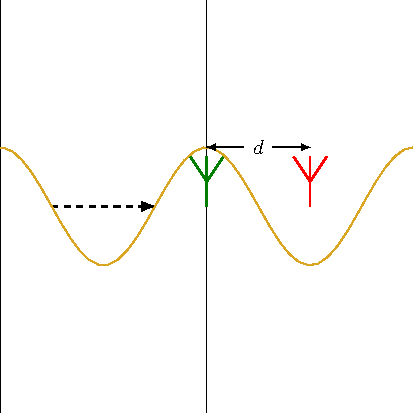
\includegraphics{../pictures/AoA_3}
            \caption*{\usebeamercolor[fg]{palette sidebar tertiary} \tiny Fonte: Autor.}
        \end{figure}
    \end{frame}

    \begin{frame}{\textit{Angle of Arrival}}
        \begin{figure}
            \centering
            \caption*{$ \theta_\text{AoA}=\SI{20}{\degree} $, $\textcolor{cmyk_M}{\alpha_{k}}=\SI{20}{\degree}$, $ \textcolor{Purple}{\beta_{\pm k}} = \SI{0}{\degree} $}
            % % \resizebox{!}{0.7\textheight}{%
\begin{circuitikz}[american, voltage shift=0.5, line width=0.5, every node/.style={font = {\footnotesize\bfseries}}]

    \def\wavelength{3.5}
    \pgfmathsetmacro\d{0.5*\wavelength}

    \def\antennaAngle{20}
    \def\signalAngle{\antennaAngle}

    \def\closeRange{9}
    \def\farRange{\closeRange+13}

	\def\NAntennas{3}
	\pgfmathsetmacro\AngleAntennas{360/\NAntennas}
	\def\ShiftAngleAntennas{-90}

	\pgfmathsetmacro\RhoAntennas{\d/(2*sin(180/\NAntennas))}

    \def\centerarc(#1)(#2:#3:#4)% Syntax: [draw options] (center) (initial angle:final angle:radius)
    { ($(#1)+({#4*cos(#2)},{#4*sin(#2)})$) arc (#2:#3:#4) }

    \def\coordref[#1](#2){%

        \coordinate(sysref) at (#2);

        \draw[#1, -latex] (sysref) ++(-0.4,-0.3) -- ++(0.9,0) node[midway, below]{$x$};
        \draw[#1, -latex] (sysref) ++(-0.3,-0.4) -- ++(0,0.9) node[midway, left]{$y$};
        \draw[#1, -latex] \centerarc(sysref)(-90:180:0.25);
        \draw[#1] (sysref) node{$+$}
    }

    \coordinate (bottomleft) at (-3.5,-1);
    \coordinate (topright) at (3.5,5);


    % \draw[Red,dashed] (bottomleft) rectangle (topright);
    \clip (bottomleft) rectangle (topright);

    \coordinate (O) at (0,0);
    \coordinate (sourceAntenna) at (\signalAngle:\closeRange*\wavelength);
    % \draw [help lines, dashed] (bottomleft) grid (topright); % desenha grid
    % \draw [red] (O) node[draw,cross out] {}; % marca pont(0,0)

    % Circulo de antenas
	% \draw[densely dotted, opacity=0.25] (O) ++(90:\RhoAntennas) circle (\RhoAntennas);

    % Linhas do sinal de fundo
    \foreach \x [evaluate={\y=int((\x+\closeRange));\z=int((\x+\closeRange));}] in {-3,...,3} {
        \draw [black!75, very thin]
        (sourceAntenna) ++ (\signalAngle:-\z*\wavelength)
            % node[anchor=west, font = {\footnotesize\bfseries}]{$\y\lambda$}
        ($(sourceAntenna) + (\signalAngle:-\z*\wavelength) + ({10*cos(\signalAngle+90)},{10*sin(\signalAngle+90)})$)
            --
        ($(sourceAntenna) + (\signalAngle:-\z*\wavelength) - ({10*cos(\signalAngle+90)},{10*sin(\signalAngle+90)})$)
        % \draw [gray, thin] (sourceAntenna) circle (\z)
        ;
    }

    % Antenas
    \draw[thick, cmyk_R] (O) node[dinantenna] (A00) {} ;
    % \draw[thick, cmyk_G, opacity=0.75] (O) ++(60:\d) node[dinantenna] (A0d) {} node [below] {$A_{k+2}$};
    \draw[thick, cmyk_B] (O) ++(\antennaAngle:\d) node[dinantenna] (Ad0) {} ;

    \draw[very thin, Black!50, -latex] % Desenha eixo X
        (-3,0) -- (3,0) node[below left] {$x$}
    ;

    % Ângulo alpha entre antenas
    \draw[thin, cmyk_M]
		(0.3,0) node [below, inner sep=3pt] {$\alpha$}
		\centerarc(O)(0:\antennaAngle:0.3)
    ;


    % Desenha senoide de fundo
    \draw[Goldenrod, domain=-8:8, samples=100]
        (A00) ++(\signalAngle+90:0.75*\wavelength) coordinate(signalAux)
        plot[shift={(signalAux)}, rotate=\signalAngle]({\x},{cos(\x * pi * 2 / \wavelength r)})
    ;

    % Direção do sinal
    \draw[very thick, dashed, -latex, Goldenrod]
        % (A00) ++(1.5*\d,0) ++ (\signalAngle:-0.25*\d) -- coordinate(angleArrow) ++(\signalAngle:0.85*\d)
        (A00) ++(-2,0) ++ (\signalAngle:-0.25*\d) -- coordinate(angleArrow) ++ (\signalAngle:0.5*\d) --++(\signalAngle:0.25*\d)
    ;
    % Angulo Theta do sinal
    \draw[thin]
        (angleArrow) ++ (0.4, 0) node [below,inner sep=2pt] {$\theta_\text{\ac{AoA}}$}
        \centerarc(angleArrow)(0:\signalAngle:0.4)
    ;

    % Triangulo retângulo + quadradinho
    \draw[Black]

    %     % (A00) --++($({\signalAngle-90}:{\d*sin(\signalAngle-\antennaAngle)})$) coordinate (pontoTriangulo) --
		(Ad0) -- (A00)

    %     % (pontoTriangulo)
    %     %   ++(\signalAngle:0.125)
    %     % --++(\signalAngle+90:0.125)
    %     % --++(\signalAngle+180:0.125)
    ;

    % % Arco do angulo beta
    % \draw[thin]
    %     \centerarc(Ad0)(180+\antennaAngle:180+\signalAngle:0.4) node[below, inner sep=3pt] {$\beta$}
    % ;

    % Distânci d entre antenas
    \draw[latex-latex]
        ($(A00)+(0,1)$) -- ($(Ad0)+(0,1)$) node [midway, fill=white, circle, inner sep=1pt] {$d$}
    ;

    \newcommand\CircleRadius{3cm}
    %   \draw (0,0) circle (\CircleRadius);
    % special method of noting the position of a point
    \coordinate (P) at (50:\CircleRadius);

\end{circuitikz}
% }


            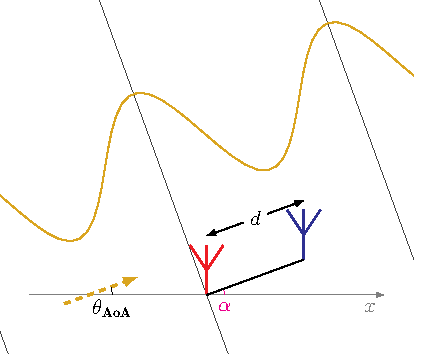
\includegraphics{../pictures/AoA_4}
            \caption*{\usebeamercolor[fg]{palette sidebar tertiary} \tiny Fonte: Autor.}
        \end{figure}
    \end{frame}

\subsection{Malha de antenas}
    \begin{frame}{Distância $d$}
                \begin{columns}
            \begin{column}{0.45\textwidth}
                \centering \vfill
                    % \resizebox{!}{0.7\textheight}{%
    \begin{circuitikz}[american, voltage shift=0.5, line width=0.5,every node/.style={font = {\footnotesize\bfseries}}]

        \def\wavelength{4}
        \def\d{0.5*\wavelength}

        \def\centerarc[#1](#2)(#3:#4:#5)% Syntax: [draw options] (center) (initial angle:final angle:radius)
        { \draw[#1] ($(#2)+({#5*cos(#3)},{#5*sin(#3)})$) arc (#3:#4:#5) node[midway,anchor=west] {$\beta$}; }

        \coordinate (bottomleft) at (-1,-1.25);
        \coordinate (topright) at (5,1.1);

        % \draw[Red,dashed] (bottomleft) rectangle (topright);
        \clip (bottomleft) rectangle (topright);

        \coordinate (O) at (0,0);
        % \draw [help lines, dashed] (-3,-3) grid (3,3); % desenha grid
        % \draw [red] (O) node[draw,cross out] {}; % marca pont(0,0)

        % \draw[Goldenrod, domain=-3:3, samples=100] plot[shift={(-1,-1)}, rotate=30]({\x},{sin(\x * pi * 2 / \wavelength r)});
        \draw[Goldenrod, domain=-3:6, samples=50]
            plot ({\x},{-cos(\x * pi * 2 / \wavelength r)})
        ;

        \draw[latex-latex]
            (0,-1.1) -- ++(\wavelength,0) node [midway, fill=white] {$\lambda$}
        ;

        \draw[Black, dashed, domain=-3:6, samples=2]
            plot[Black, thin, dashed, samples=2] (\x,0)
        ;

        \pause
        \draw[thick]
            (2,0)  node[cmyk_B, dinantenna] (A00) {}
        ;

        \pause
        \draw[thick]
            (-0,0) node[cmyk_R,   dinantenna] (Ad0) {}
        ;

    \visible<3-6>{
        \draw[latex-latex]
            ($(A00)+(0,-0.1)$) -- ++(-\d,0) node [midway, fill=white, fill opacity=0.75, anchor=north] {$d$}
        ;
    }

    \visible<7->{
        \draw[latex-latex]
            ($(A00)+(0,-0.1)$) -- ++(-\d,0) node [midway, fill=white, fill opacity=0.75, anchor=north] {$d = \sfrac{\lambda}{2}$}
        ;
    }

    \end{circuitikz}
  % }\vfill
                \visible<5->{    % \resizebox{!}{0.7\textheight}{%
    \begin{circuitikz}[american, voltage shift=0.5, line width=0.5,every node/.style={font = {\footnotesize\bfseries}}]

        \def\wavelength{4}
        \def\d{0.5*\wavelength}


        \def\antennaAngle{120}
        \def\closeRange{9}
        \def\farRange{\closeRange+13}

        \def\centerarc[#1](#2)(#3:#4:#5)% Syntax: [draw options] (center) (initial angle:final angle:radius)
        { \draw[#1] ($(#2)+({#5*cos(#3)},{#5*sin(#3)})$) arc (#3:#4:#5) node[midway,anchor=west] {$\beta$}; }


        \coordinate (O) at (0,0);
        \coordinate (antenna) at (\antennaAngle:\closeRange*\wavelength);
        % \draw [help lines, dashed] (-3,-3) grid (3,3); % desenha grid
        % \draw [red] (O) node[draw,cross out] {}; % marca pont(0,0)

        % \draw (-6.8,-4) rectangle (6.8,4);
        \clip (-1,-1.1) rectangle (5,1.1);


        \draw[thick]
            (0,0)  node[cmyk_B, dinantenna] (A00) {}
            % (0,\d) node[Blue,  dinantenna] (A0d) {}
            (1.2*\d,0) node[cmyk_R,   dinantenna] (Ad0) {}
            (0.8*\d,0) node[cmyk_R,   dinantenna, opacity=0.2] (Ad0_phantom) {}
        ;

        % \draw[Goldenrod, domain=-3:3, samples=100] plot[shift={(-1,-1)}, rotate=30]({\x},{sin(\x * pi * 2 / \wavelength r)});
        \draw[Goldenrod, domain=-3:6, samples=50]
            plot ({\x},{cos(\x * pi * 2 / \wavelength r)})
        ;

        \draw[Black, dashed, domain=-3:6, samples=2]
            plot[Black, thin, dashed, samples=2] (\x,0)
        ;

        \draw [densely dotted, cmyk_R]
            (Ad0_phantom) --
            ++(0,{cos(1.2*\d * pi * 2 / \wavelength r)}) --
            ++({0.4*\d},0) --
            (Ad0)
        ;

    \end{circuitikz}
  % }}\vfill
                \visible<6->{    % \resizebox{!}{0.7\textheight}{%
    \begin{circuitikz}[american, voltage shift=0.5, line width=0.5,every node/.style={font = {\footnotesize\bfseries}}]

        \def\wavelength{4}
        \def\d{0.5*\wavelength}

        \def\centerarc[#1](#2)(#3:#4:#5)% Syntax: [draw options] (center) (initial angle:final angle:radius)
        { \draw[#1] ($(#2)+({#5*cos(#3)},{#5*sin(#3)})$) arc (#3:#4:#5) node[midway,anchor=west] {$\beta$}; }

        \coordinate (bottomleft) at (-1,-1.25);
        \coordinate (topright) at (5,1.1);

        % \draw[Red,dashed] (bottomleft) rectangle (topright);
        \clip (bottomleft) rectangle (topright);

        \coordinate (O) at (0,0);
        % \draw [help lines, dashed] (bottomleft) grid (topright); % desenha grid
        % \draw [red] (O) node[draw,cross out] {}; % marca pont(0,0)

        \pgfmathsetmacro\vCos{-cos(-0.5*pi*2/\wavelength r)}

        \draw[thick]
            (2,0)  node[cmyk_B, dinantenna] (A00) {}
            % (0,\d) node[Blue,  dinantenna] (A0d) {}
            (0.5,0) node[cmyk_R,   dinantenna] (Ad0) {}
            % (3.5,0) node[cmyk_R,   dinantenna, opacity=0.2] (Ad0_phantom) {}
        ;

        % \draw[Goldenrod, domain=-3:3, samples=100] plot[shift={(-1,-1)}, rotate=30]({\x},{sin(\x * pi * 2 / \wavelength r)});
        \draw[Goldenrod, domain=-3:6, samples=50]
            plot ({\x},{-cos(\x * pi * 2 / \wavelength r)})
        ;

        \draw[Black, dashed, domain=-3:6, samples=2]
            plot[Black, thin, dashed, samples=2] (\x,0)
        ;

    \end{circuitikz}
  % }}\vfill
            \end{column}
            \begin{column}{0.55\textwidth}
                \begin{itemize}[<+(-1)->]\addtolength{\itemsep}{0.5\baselineskip}
                    \item Toma-se uma \textcolor{cmyk_B}{antena} como referência
                    \item Posiciona-se uma \textcolor{Red}{segunda antena} a uma distância $d$ determinada
                    \item Analisando a defasagem entre as antenas, é possível determinar o ângulo de incidência do sinal
                    \item Se a distância for maior que $\sfrac{\lambda}{2}$, haverá conflito de defasagem
                    \item Se for menor, há perda de resolução
                    \item Adota-se a distância de $d = \sfrac{\lambda}{2}$
                \end{itemize}
            \end{column}
        \end{columns}
    \end{frame}

    \begin{frame}{Geometria da malha de antenas}
        \begin{equation*}
            \rho = \frac{d}{2\cdot \sin\left(\displaystyle\frac{\pi}{N_\text{ant}}\right)}
        \end{equation*}

        \begin{equation*}
            k = \left\{1, 2, \dotsc, N_\text{ant}\right\}
        \end{equation*}

        \begin{equation*}
            \textcolor{cmyk_B}{A_k} =
            \rho
            \cdot \exp\left(\imath\cdot k \cdot \frac{2\pi}{N_\text{ant}}\right) =
            \left( \operatorname{\mathcal{Re}}\left( \textcolor{cmyk_B}{A_k} \right), ~\operatorname{\mathcal{Im}}\left( \textcolor{cmyk_B}{A_k} \right) \right) =
            \left( x_{A_k}, ~ y_{A_k} \right)
        \end{equation*}

        \begin{equation*}
            \textcolor{cmyk_M}{\alpha_k} = \arg\left( \textcolor{cmyk_B}{A_k} - \textcolor{cmyk_R}{A_{k+1}} \right)
        \end{equation*}
    \end{frame}

    \begin{frame}{Três antenas}
        \centering%
        % \fbox{%
            % \scalebox{0.75}%
            % \resizebox{0.5\textwidth}{!}
            % {% \resizebox{!}{0.7\textheight}{%
\begin{circuitikz}[american, voltage shift=0.5, line width=0.5,every node/.style={font = {\footnotesize\bfseries}}]

    \def\wavelength{8}
    \pgfmathsetmacro\d{0.5*\wavelength}

    \def\signalAngle{75}
    \def\antennaAngle{120}

    \def\closeRange{9}
    \def\farRange{\closeRange+13}

	\def\NAntennas{3}
	\pgfmathsetmacro\AngleAntennas{360/\NAntennas}
	\def\ShiftAngleAntennas{-90}

	\pgfmathsetmacro\RhoAntennas{\d/(2*sin(180/\NAntennas))}

    \def\centerarc(#1)(#2:#3:#4)% Syntax: [draw options] (center) (initial angle:final angle:radius)
    { ($(#1)+({#4*cos(#2)},{#4*sin(#2)})$) arc (#2:#3:#4) }

    \def\coordref[#1](#2){%

        \coordinate(sysref) at (#2);

        \draw[#1, -latex] (sysref) ++(-0.4,-0.3) -- ++(0.9,0) node[midway, below]{$x$};
        \draw[#1, -latex] (sysref) ++(-0.3,-0.4) -- ++(0,0.9) node[midway, left]{$y$};
        \draw[#1, -latex] \centerarc(sysref)(-90:180:0.25);
        \draw[#1] (sysref) node{$+$}
    }

    \coordinate (bottomleft) at (-3,-3);
    \coordinate (topright) at (3,3);


    % \draw[Red,dashed] (bottomleft) rectangle (topright);
    \clip (bottomleft) rectangle (topright);

    \coordinate (O) at (0,0);
    \coordinate (sourceAntenna) at (\signalAngle:\closeRange*\wavelength);
    % \draw [help lines, dashed] (bottomleft) grid (topright); % desenha grid
    % \draw [red] (O) node[draw,cross out] {}; % marca pont(0,0)

	\draw[densely dotted] (O) circle (\RhoAntennas);

    \draw[thick, cmyk_G] (O) ++(1*\AngleAntennas+\ShiftAngleAntennas:\RhoAntennas) node[dinantenna] (A1) {} node [above right] {$A_{1}$};
    \draw[thick, cmyk_B] (O) ++(2*\AngleAntennas+\ShiftAngleAntennas:\RhoAntennas) node[dinantenna] (A2) {} node [above left] {$A_{2}$};
    \draw[thick, cmyk_R] (O) ++(3*\AngleAntennas+\ShiftAngleAntennas:\RhoAntennas) node[dinantenna] (A3) {};

	\coordinate (A1_2) at ($(A1)!0.5!(A2)$);

	\draw[Black!25, dotted]
		(A1) --
		(A3) --
		(A2)
	;

	\draw[Black!50, densely dotted]
		(O) --
		(A2) --
		(A1_2)
	;

	\draw
		(A1) --
		(O) --
		(A1_2) --
		(A1)
	;

	\draw
         (A1_2)
           ++(0:0.125)
         --++(-90:0.125)
         --++(+180:0.125)
	;

	\node at (O) {\tiny\textbullet};

	\draw
		(O) ++(90:0.3) node[left, inner sep=1.5pt] {$\textstyle \frac{\pi}{N_\text{ant}}$}
		\centerarc(O)(1*\AngleAntennas+\ShiftAngleAntennas:90:0.3)
	;


    % Distânci d entre antenas
    \draw[latex-latex]
        ($(A1)+(0,1)$) -- ($(A2)+(0,1)$) node [midway, fill=white, circle, inner sep=1pt] {$d$}
    ;

    \draw[decorate, decoration={brace, amplitude=5pt}, thin]
    ($(A1)+({1*\AngleAntennas+\ShiftAngleAntennas-90}:0.1)$)
    -- coordinate (brace)
    ($(O)+({1*\AngleAntennas+\ShiftAngleAntennas-90}:0.1)$)
    ;

    \draw (brace) ++({1*\AngleAntennas+\ShiftAngleAntennas-90}:5pt)
        node[anchor=north west, circle, fill=white, inner sep=1pt] {$\rho$}
    ;

	\draw[decorate, decoration={brace, amplitude=5pt}, thin]
    ($(A1_2)+({90}:0.1)$)
    -- coordinate (brace)
    ($(A1)+({90}:0.1)$)
    ;

    \draw (brace) ++({90}:5pt)
        node[anchor=south, circle, inner sep=1pt] {$\sfrac{d}{2}$}
    ;

    % \coordref[Black!25](3.5,0);

\end{circuitikz}
% }

}%
            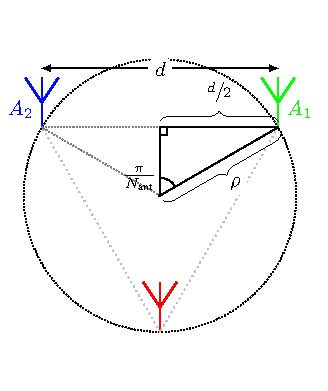
\includegraphics[scale=0.8]{../pictures/antennas_3.pdf}%
        % }
        % \vfill
    \end{frame}
    \begin{frame}{Cinco antenas}
        \centering%
        % \fbox{%
            % \scalebox{0.75}%
            % \resizebox{0.5\textwidth}{!}
            % {% \resizebox{!}{0.7\textheight}{%
\begin{circuitikz}[american, voltage shift=0.5, line width=0.5,every node/.style={font = {\footnotesize\bfseries}}]

    \def\wavelength{8}
    \pgfmathsetmacro\d{0.5*\wavelength}

    \def\signalAngle{75}
    \def\antennaAngle{120}

    \def\closeRange{9}
    \def\farRange{\closeRange+13}

	\def\NAntennas{5}
	\pgfmathsetmacro\AngleAntennas{360/\NAntennas}
	\pgfmathsetmacro\ShiftAngleAntennas{-90+\AngleAntennas}

	\pgfmathsetmacro\RhoAntennas{\d/(2*sin(180/\NAntennas))}

    \def\centerarc(#1)(#2:#3:#4)% Syntax: [draw options] (center) (initial angle:final angle:radius)
    { ($(#1)+({#4*cos(#2)},{#4*sin(#2)})$) arc (#2:#3:#4) }

    \def\coordref[#1](#2){%

        \coordinate(sysref) at (#2);

        \draw[#1, -latex] (sysref) ++(-0.4,-0.3) -- ++(0.9,0) node[midway, below]{$x$};
        \draw[#1, -latex] (sysref) ++(-0.3,-0.4) -- ++(0,0.9) node[midway, left]{$y$};
        \draw[#1, -latex] \centerarc(sysref)(-90:180:0.25);
        \draw[#1] (sysref) node{$+$}
    }

    \coordinate (bottomleft) at (-4,-4);
    \coordinate (topright) at (4,4);


    % \draw[Red,dashed] (bottomleft) rectangle (topright);
    \clip (bottomleft) rectangle (topright);

    \coordinate (O) at (0,0);
    \coordinate (sourceAntenna) at (\signalAngle:\closeRange*\wavelength);
    % \draw [help lines, dashed] (bottomleft) grid (topright); % desenha grid
    % \draw [red] (O) node[draw,cross out] {}; % marca pont(0,0)

	\draw[densely dotted] (O) circle (\RhoAntennas);

    \draw[thick, cmyk_G] (O) ++(1*\AngleAntennas+\ShiftAngleAntennas:\RhoAntennas) node[dinantenna] (A1) {} node [above right] {$A_{1}$};
    \draw[thick, cmyk_B] (O) ++(2*\AngleAntennas+\ShiftAngleAntennas:\RhoAntennas) node[dinantenna] (A2) {} node [above left] {$A_{2}$};
    \draw[thick, cmyk_R] (O) ++(3*\AngleAntennas+\ShiftAngleAntennas:\RhoAntennas) node[dinantenna] (A3) {};
    \draw[thick, cmyk_C] (O) ++(4*\AngleAntennas+\ShiftAngleAntennas:\RhoAntennas) node[dinantenna] (A4) {};
    \draw[thick, cmyk_M] (O) ++(5*\AngleAntennas+\ShiftAngleAntennas:\RhoAntennas) node[dinantenna] (A5) {};

	\coordinate (A1_2) at ($(A1)!0.5!(A2)$);

	\draw[Black!25, dotted]
		(A1) --
		(A5) --
		(A4) --
		(A3) --
		(A2)
	;

	\draw[Black!50, densely dotted]
		(O) --
		(A2) --
		(A1_2)
	;

	\draw
		(A1) --
		(O) --
		(A1_2) --
		(A1)
	;

	\draw
         (A1_2)
           ++(0:0.125)
         --++(-90:0.125)
         --++(+180:0.125)
	;

	\node at (O) {\tiny\textbullet};

	\draw
		(O) ++(90:0.3) node[left, inner sep=1.5pt] {$\textstyle \frac{\pi}{N_\text{ant}}$}
		\centerarc(O)(1*\AngleAntennas+\ShiftAngleAntennas:90:0.3)
	;


    % Distânci d entre antenas
    \draw[latex-latex]
        ($(A1)+(0,1)$) -- ($(A2)+(0,1)$) node [midway, fill=white, circle, inner sep=1pt] {$d$}
    ;

    \draw[decorate, decoration={brace, amplitude=5pt}, thin]
    ($(A1)+({1*\AngleAntennas+\ShiftAngleAntennas-90}:0.1)$)
    -- coordinate (brace)
    ($(O)+({1*\AngleAntennas+\ShiftAngleAntennas-90}:0.1)$)
    ;

    \draw (brace) ++({1*\AngleAntennas+\ShiftAngleAntennas-90}:5pt)
        node[anchor=north west, circle, fill=white, inner sep=1pt] {$\rho$}
    ;

	\draw[decorate, decoration={brace, amplitude=5pt}, thin]
    ($(A1_2)+({90}:0.1)$)
    -- coordinate (brace)
    ($(A1)+({90}:0.1)$)
    ;

    \draw (brace) ++({90}:5pt)
        node[anchor=south, circle, inner sep=1pt] {$\sfrac{d}{2}$}
    ;

    % \coordref[Black!25](3.5,0);

\end{circuitikz}
% }

}%
            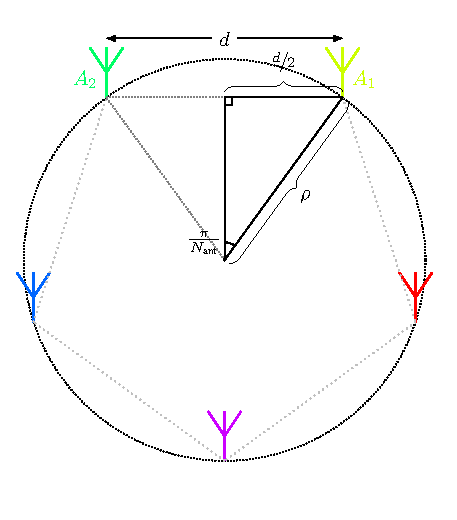
\includegraphics[scale=0.8]{../pictures/antennas_5.pdf}%
        % }
        % \vfill
    \end{frame}
    \begin{frame}{Sete antenas}
        \centering%
        % \fbox{%
            % \scalebox{0.75}%
            % \resizebox{0.5\textwidth}{!}
            % {% \resizebox{!}{0.7\textheight}{%
\begin{circuitikz}[american, voltage shift=0.5, line width=0.5,every node/.style={font = {\footnotesize\bfseries}}]

    \def\wavelength{8}
    \pgfmathsetmacro\d{0.5*\wavelength}

    \def\signalAngle{75}
    \def\antennaAngle{120}

    \def\closeRange{9}
    \def\farRange{\closeRange+13}

	\def\NAntennas{7}
	\pgfmathsetmacro\AngleAntennas{360/\NAntennas}
	\pgfmathsetmacro\ShiftAngleAntennas{-90+2*\AngleAntennas}

	\pgfmathsetmacro\RhoAntennas{\d/(2*sin(180/\NAntennas))}

    \def\centerarc(#1)(#2:#3:#4)% Syntax: [draw options] (center) (initial angle:final angle:radius)
    { ($(#1)+({#4*cos(#2)},{#4*sin(#2)})$) arc (#2:#3:#4) }

    \def\coordref[#1](#2){%

        \coordinate(sysref) at (#2);

        \draw[#1, -latex] (sysref) ++(-0.4,-0.3) -- ++(0.9,0) node[midway, below]{$x$};
        \draw[#1, -latex] (sysref) ++(-0.3,-0.4) -- ++(0,0.9) node[midway, left]{$y$};
        \draw[#1, -latex] \centerarc(sysref)(-90:180:0.25);
        \draw[#1] (sysref) node{$+$}
    }

    \pgfmathsetmacro\vSize{\RhoAntennas + 1}
    \pgfmathsetmacro\hSize{\RhoAntennas + 0.4}

    \coordinate (bottomleft) at (-\hSize,-\vSize);
    \coordinate (topright) at (\hSize,\vSize);

    % \draw[Red, thick]
    %     (bottomleft) -- (topright)
    %     (\hSize,-\vSize) -- (-\hSize,\vSize)
    % ;

    % \draw[Red,dashed] (bottomleft) rectangle (topright);
    \clip (bottomleft) rectangle (topright);

    \coordinate (O) at (0,0);
    \coordinate (sourceAntenna) at (\signalAngle:\closeRange*\wavelength);
    % \draw [help lines, dashed] (bottomleft) grid (topright); % desenha grid
    % \draw [red] (O) node[draw,cross out] {}; % marca pont(0,0)

	\draw[densely dotted] (O) circle (\RhoAntennas);

    \draw[thick, antena_7_1] (O) ++(1*\AngleAntennas+\ShiftAngleAntennas:\RhoAntennas) node[dinantenna] (A1) {} node [above right] {$A_{1}$};
    \draw[thick, antena_7_2] (O) ++(2*\AngleAntennas+\ShiftAngleAntennas:\RhoAntennas) node[dinantenna] (A2) {} node [above left] {$A_{2}$};
    \draw[thick, antena_7_3] (O) ++(3*\AngleAntennas+\ShiftAngleAntennas:\RhoAntennas) node[dinantenna] (A3) {};
    \draw[thick, antena_7_4] (O) ++(4*\AngleAntennas+\ShiftAngleAntennas:\RhoAntennas) node[dinantenna] (A4) {};
    \draw[thick, antena_7_5] (O) ++(5*\AngleAntennas+\ShiftAngleAntennas:\RhoAntennas) node[dinantenna] (A5) {};
    \draw[thick, antena_7_6] (O) ++(6*\AngleAntennas+\ShiftAngleAntennas:\RhoAntennas) node[dinantenna] (A6) {};
    \draw[thick, antena_7_7] (O) ++(7*\AngleAntennas+\ShiftAngleAntennas:\RhoAntennas) node[dinantenna] (A7) {};

	\coordinate (A1_2) at ($(A1)!0.5!(A2)$);

	\draw[Black!25, dotted]
		(A1) --
		(A7) --
		(A6) --
		(A5) --
		(A4) --
		(A3) --
		(A2)
	;

	\draw[Black!50, densely dotted]
		(O) --
		(A2) --
		(A1_2)
	;

	\draw
		(A1) --
		(O) --
		(A1_2) --
		(A1)
	;

	\draw
         (A1_2)
           ++(0:0.125)
         --++(-90:0.125)
         --++(+180:0.125)
	;

	\node at (O) {\tiny\textbullet};

	\draw
		(O) ++(90:0.3) node[left, inner sep=1.5pt] {$\textstyle \frac{\pi}{N_\text{ant}}$}
		\centerarc(O)(1*\AngleAntennas+\ShiftAngleAntennas:90:0.3)
	;


    % Distânci d entre antenas
    \draw[latex-latex]
        ($(A1)+(0,1)$) -- ($(A2)+(0,1)$) node [midway, fill=white, circle, inner sep=1pt] {$d$}
    ;

    \draw[decorate, decoration={brace, amplitude=5pt}, thin]
    ($(A1)+({1*\AngleAntennas+\ShiftAngleAntennas-90}:0.1)$)
    -- coordinate (brace)
    ($(O)+({1*\AngleAntennas+\ShiftAngleAntennas-90}:0.1)$)
    ;

    \draw (brace) ++({1*\AngleAntennas+\ShiftAngleAntennas-90}:5pt)
        node[anchor=north west, circle, fill=white, inner sep=1pt] {$\rho$}
    ;

	\draw[decorate, decoration={brace, amplitude=5pt}, thin]
    ($(A1_2)+({90}:0.1)$)
    -- coordinate (brace)
    ($(A1)+({90}:0.1)$)
    ;

    \draw (brace) ++({90}:5pt)
        node[anchor=south, circle, inner sep=1pt] {$\sfrac{d}{2}$}
    ;

    % \coordref[Black!25](3.5,0);

\end{circuitikz}
% }

}%
            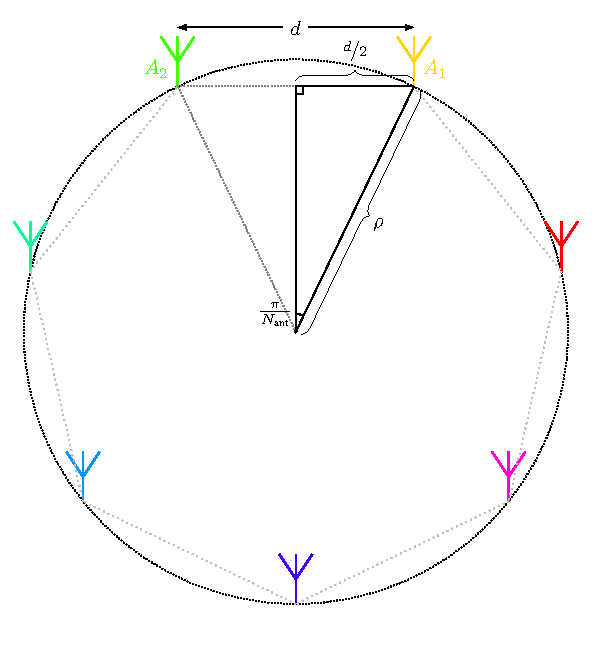
\includegraphics[scale=0.8]{../pictures/antennas_7.pdf}%
        % }
        % \vfill
    \end{frame}

\subsection{Calculo de fase}
    \begin{frame}{Cálculo de defasagem}
        \begin{equation*}
            T = \frac{2\pi}{\omega} = \frac{1}{f}
        \end{equation*}

        \begin{equation*}
            I_k =
            \int\limits_0^{T} \cos\left(\omega \cdot\tau\right)
            \cdot w\left( x_{A_k}, ~y_{A_k}, ~\tau \right) \partial \tau
        \end{equation*}

        \begin{equation*}
            Q_k =
            \int\limits_0^{T} \sin\left(\omega\cdot\tau\right)
            \cdot w\left( x_{A_k}, ~y_{A_k}, ~\tau \right) \partial \tau
        \end{equation*}

        \begin{equation*}
            \textcolor{cmyk_B}{Z_k} =
            \frac{\omega}{\pi}\cdot\left(I_k + \imath Q_k\right)
        \end{equation*}

        \begin{equation*}
            \Delta_\Phi =
            \textcolor{cmyk_B}{\Phi_k} - \textcolor{cmyk_R}{\Phi_{k+1}} =
            \arg\left(\textcolor{cmyk_B}{Z_k}\right) - \arg\left(\textcolor{cmyk_R}{Z_{k+1}}\right) =
            \arg\left(\textcolor{cmyk_B}{Z_k} \cdot \overline{\textcolor{cmyk_R}{Z_{k+1}}}\right)
        \end{equation*}

        \begin{equation*}
            \textcolor{Purple}{\beta_{\pm k}} = \arccos\left(\frac{\cancel{\lambda}}{\cancel{d}}\cdot\frac{\Delta_\Phi}{\cancel{2}\pi}\right)
        \end{equation*}

    \end{frame}

    \begin{frame}{Geometria do sistema}
        \centering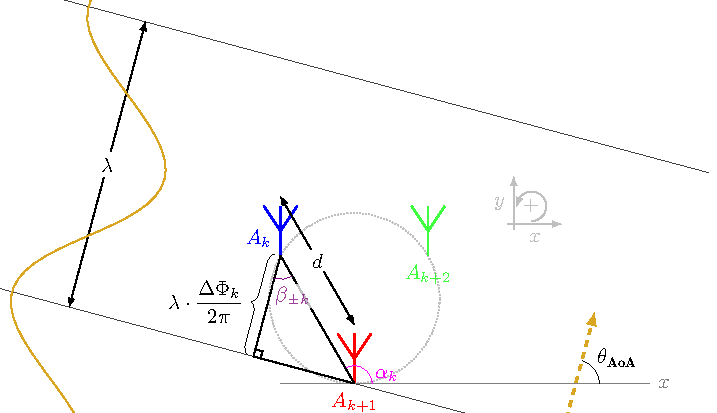
\includegraphics{../pictures/AoA_geometria.pdf}
    \end{frame}

\subsection{Determinar AoA}
    \begin{frame}{Determinar AoA}
        \begin{equation*}
            \theta_{\pm k} = \textcolor{cmyk_M}{\alpha_k}\pm \textcolor{Purple}{\beta_{\pm k}}
        \end{equation*}

        \begin{equation*}
            \Theta = \left\{\theta_{\pm k} ~\middle\vert~ \forall k\right\}
        \end{equation*}

        \begin{equation*}
            \delta = \frac{\pi}{2 \cdot \left( 1 + N_\text{ant} \right)}
        \end{equation*}

        \begin{equation*}
            \Theta_{\left\lfloor\bullet\right\rceil} =
            \left\{\left\lfloor\frac{\theta}{\delta}\right\rceil\cdot\delta ~\middle\vert~ \forall \theta \in \Theta  \right\}
        \end{equation*}

        \begin{equation*}
            \theta_\mathcal{M_o} = \operatorname{\mathcal{M_o}}\left( \Theta_{\left\lfloor\bullet\right\rceil}  \right)
        \end{equation*}

        \begin{equation*}
            \Theta_\text{F} = \left\{\theta \in \Theta  ~\middle\vert~
            \theta_\mathcal{M_o} - \delta \leq \theta \leq \theta_\mathcal{M_o} + \delta\right\}
        \end{equation*}

        \begin{equation*}
            \theta_\text{AoA} = \widetilde{\Theta_\text{F}}
        \end{equation*}
    \end{frame}


    % \begin{frame}{\href{https://drive.google.com/file/d/1-ep5hH8TSrnHU_m9b4AFmUJlB_hGR41m/view?usp=drive_link}{Análise de vetores complexos}}
    %     % \begin{multicols}{2}
    %         \begin{equation*}
    %             C(x,y) = \int_0^T w(x,y,t) \cdot \cos(k(x,y,t)) \partial t
    %         \end{equation*}

    %         \begin{equation*}
    %             S(x,y) = \int_0^T w(x,y,t) \cdot \sin(k(x,y,t)) \partial t
    %         \end{equation*}

    %         \begin{equation*}
    %             Z(x,y) = 2\cdot(S + \imath C)
    %         \end{equation*}

    %         \begin{equation*}
    %             \Delta_{x,y} = \arg(\textcolor{Green}{Z_{0,0}}\cdot Z^*_{x,y})
    %         \end{equation*}

    %         \begin{equation*}
    %             \text{componente}_{x,y} = -\frac{\Delta_{x,y}}{\pi}\cdot\frac{\cancel{\lambda}}{\cancel{d \cdot 2}} = -\frac{\Delta_{x,y}}{\pi}
    %         \end{equation*}
    %         % \end{multicols}
    % \end{frame}